
%-----------------------------------------------------------------------------
% FV Optimization
%-----------------------------------------------------------------------------
\section{Optimization of fiTQun Fiducial Volume Cuts}
\label{sec:fvopt}


%-----------------------------------------------------------------------------
% Intro
%-----------------------------------------------------------------------------
\subsection{Introduction}
\label{subsec:fvintro}


Since the fiTQun algorithm represents a fundamental change in the SK
reconstruction methods, a new set of optimization studies must be performed to
determine the best event selection cuts for the T2K oscillation analyses.
The optimization of the topological cuts that separate the T2K \numu and \nue
events are described in detail in TN-319~\cite{tn319}. In this section
we will describe a separate analysis for determining the fiducial volume (FV) cuts for each
T2K sample.  

The choice of FV cuts for the fiTQun T2K event selections presents a formidable
optimization problem. As the FV cuts are loosened, more neutrino events are
allowed into the T2K samples, which improves the statistical constraint on the
oscillation parameters.  However, accepting events from regions near the inner
detector (ID) wall may also introduce additional backgrounds that counteract
any statistical gain.  Further complicating the situation is the presence of
systematic uncertainties, which may be larger in regions near the ID wall and
also potentially offset any statistical gain in sensitivity.

The overall approach to this problem is to define a figure of merit that
approximates the sensitivity to the neutrino oscillation parameters in the
presence of the estimated systematics. The systematics in various detector
regions are then constrained use the results of the atmospheric neutrino fit
described in Section~\ref{sec:methods}.  The FV cuts for each T2K sample are 
then taken to be the cuts that maximize this figure of merit (subject to some
constraints). Each T2K selection faces a different set of backgrounds near the ID
wall, so the FV cuts for each sample are estimated separately.  The optimized cuts
are then applied to each selection for both FHC and RHC modes


%-----------------------------------------------------------------------------
% Figure of Merit
%-----------------------------------------------------------------------------
\subsection{Figure of Merit}
\label{subsec:metric}


The determination of the ``optimal'' fiducial volume cuts requires a
quantitative definition of ``optimal''.  Ideally, the quantity we would like to
optimize is the sensitivity to the underlying neutrino oscillation parameters,
(and indeed future optimization analyses should strive to do this), but the
precise determination of the sensitivity is itself a complex analyses that does
not lend itself well to repeated sampling under varying FV cut assumptions.
For this analysis, we choose instead to use a simple numerical figure of merit
as our optimization metric.  At minimum, the figure of merit should try to
account for the competing effects of statistics, purity and uncertainty. 

The FV optimization figure of merit can be derived by maximizing the
sensitivity for a very simplified parameter estimation framework. We
consider the likelihood of observing $X$ events in some Poisson process whose
mean depends on an underlying parameter $\theta$. Clearly, for the T2K
analysis, $X$ represents the observed number of neutrino events in some sample,
and $\theta$ represents the corresponding oscillation parameter of interest
(i.e. \thdis or \dcp).  If we expect $X>10$ we may approximate the probability
of observing $X$ given $\theta$ to be Gaussian, so the corresponding likelihood
is:
%
\begin{equation}
  -log[\mathcal{L}(X|\theta)] \approx \frac{(X - N(\theta))^{2}}{2\sigma^{2}}
\end{equation}
%
where $N(\theta)$ is the Poisson mean as a function of $\theta$, and $\sigma$
is some measure of the uncertainty associated in measuring $X$ that will be
quantified later. The sensitivity to the parameter  $\theta$ depends on the
curvature of the likelihood, which can be expressed as:
%
\begin{equation}
\label{eq:lderiv}
  -\frac{\partial^{2}  log[\mathcal{L}(X|\theta)]}{\partial \theta^{2}} =
  \frac{1}{\sigma^{2}}\bigg[(X - N)\frac{\partial^{2} N}{\partial \theta^{2}} - \bigg(\frac{\partial N}{\partial \theta}\bigg)^{2} \bigg]
\end{equation}
%
We assume the observed data $X$ is drawn from a Poisson distribution with a
mean $N(\theta_{true})$.  The expectation value of the curvature at the true
parameter value over an ensemble of hypothetical measurements can then be
expressed as:
%
\begin{equation}
  \bigg\langle \frac{\partial^{2} log[\mathcal{L}(X|\theta)]}{\partial \theta^{2}} \Big|_{\theta = \theta_{true}}  \bigg\rangle_{X} = 
  \frac{\big( \frac{\partial N}{\partial \theta}|_{\theta = \theta_{true}}\big)^{2}}{\sigma^{2}}
\end{equation}
%
Where we see the first term in Equation~\ref{eq:lderiv} vanishes since X varies
symmetrically about the true mean.  We now make the assumption that the total
uncertainty can be expressed as a quadrature sum the Poisson statistical
uncertainty and the systematic uncertainty inherent to our measurement, so
$\sigma^{2} = N + \sigma^{2}_{syst}$.  The expected curvature then becomes:
%
\begin{equation}
   \bigg\langle \frac{\partial^{2} log[\mathcal{L}(X|\theta)]}{\partial \theta^{2}} \Big|_{\theta = \theta_{true}}  \bigg\rangle_{X} = 
   \frac{\big( \frac{\partial N}{\partial \theta}|_{\theta = \theta_{true}}\big)^{2}}{N(\theta_{true}) + \sigma_{syst}^{2}}
\end{equation}
%
In practice, we can apply this equation to the T2K analysis by noting that the
T2K MC predicts an expected number of events that we believe best approximates
$N(\theta_{true})$, so if we let $\hat{N}$ be the MC prediction we obtain as a
figure of merit:
%
\begin{equation}
\label{eq:fom}
  F.O.M = \frac{\big( \frac{\partial \hat{N}}{\partial \theta}\big)^{2}}{\hat{N} + \sigma_{syst}^{2}}
\end{equation}
%
This figure of merit makes intuitive sense, we wish to maximize the change in
our expected number of events with respect to the underlying oscillation
parameter, divided by the total uncertainty.  The numerator can be calculated
easily from the known oscillation probabilities, and is effectively a small
correction to put emphasis on events with energies near the maximum oscillation
signal. To calculate the denominator, we must obtain some estimate of the
systematic uncertainties in various detector regions from the atmospheric
neutrino fit.



%-----------------------------------------------------------------------------
% Uncertainties in Detector Regions
%-----------------------------------------------------------------------------
\subsection{Systematic Uncertainty in SK Detector Regions}
\label{subsec:fvunc}

To evaluate the figure of merit expressed in Equation~\ref{eq:fom} for various
assumptions of FV cuts, we must estimate how the systematic uncertainty behaves
in each detector region.  To accomplish this, the detector is binned into
various \wall and \towall regions according to Section~\ref{subsec:DR}.  This
binning was chosen to isolate regions where the detector systematics may differ
from those near the center of the tank, while also being large enough to
provide a constraint from limited atmospheric neutrino data.  In each detector
region, we break down the systematic uncertainty as the uncertainty in the
number events that pass our selection criteria in three broad event categories: 

\begin{table}
  \centering
  \begin{tabular}{l | l |l}
  \hline\hline
  Category \# & Category Name & Definition \\
  \hline
  0 & CCQE & True CCQE interaction \\
  1 & CCnQE & True CC interaction that is not CCQE \\
  2 & CCmisID & True CC interaction from the wrong neutrino flavor \\
  3 & NC & True NC interaction \\
  4 & Entering & True \wall $< 0$ \\
  \hline\hline
  \end{tabular}
  \caption{List of the MC signal and background catagories that are used for each
  T2K event selection in the fiducial volume optimizaton studies.}
  \label{tab:cat}
\end{table}

To estimate the detector systematic uncertainty in each of these regions, we
utilize the results of the atmospheric fit described in
Section~\ref{sec:methods}. This is done by building a distribution of the
number of events in each region for a series of toy experiments using following
procedure:

\begin{enumerate}
  \item Choose a random sample histogram shape parameters from posterior Markov chain.
  \item Loop over the T2K MC events, and for each event directly modify the fiTQun cut variables
    according to Equation~\ref{eq:fqparmod}.
  \item Check if the modified event passes any of the T2K event selection cuts,
    if it passes, add it to a running
    count of number events for each category in each detector region.
  \item Repeat from Step 1 until a suitable number of toy samples have been generated
\end{enumerate}

The result after following this procedure is a set of distributions of toy
samples for each detector region and for each of the signal and background
categories in Table~\ref{tab:cat}.  An example of one such distribution is
shown in Figure~\ref{fig:fverrsinglebin}.  For each distribution, two important
quantities are calculated.  The first quantity is the fractional deviation of
the mean of the distribution of toy experiments from the nominal MC value.
This is referred to as the ``shift error'' and represents the size of the
difference between the MC simulation and what we expect from data.  The second
quantity is the square root of the variance of the distribution of toy
experiments.  This is referred to as the ``fit error'' and represents the
statistical uncertainty of our measurement of the deviation from the true MC
value.  The total error in each detector region and for each MC category in
Table~\ref{tab:cat} is then quoted as the quadrature sum of the fit error and
the shift error. 

\begin{figure}[h]
  \begin{center}
    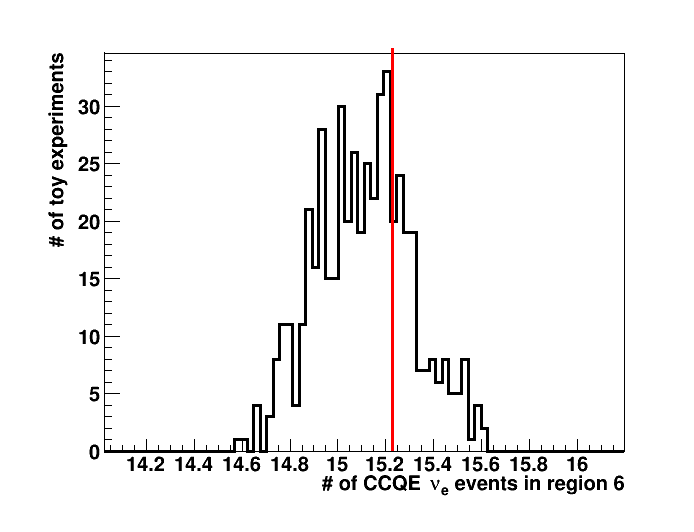
\includegraphics[width=0.6\textwidth]{dist_example}
  \end{center}
  \caption{This figure shows an example of one of the distributions that are
  used to calculate the detector systematic uncertainties in each FV bin.  The
  ``fit error'' is calculated from the width of this distribution, while the
  ``shift error'' is calculated from the difference between the distribution
  mean and the nominal MC value (red line).  The total uncertainty in each
  detector region in Figures~\ref{fig:fverrnue}-\ref{fig:fverrnue1rpi} is the
  quadrature of sum of the ``fit error''.}
  \label{fig:fverrsinglebin}
\end{figure}

\begin{figure}[h]
  \begin{center}
    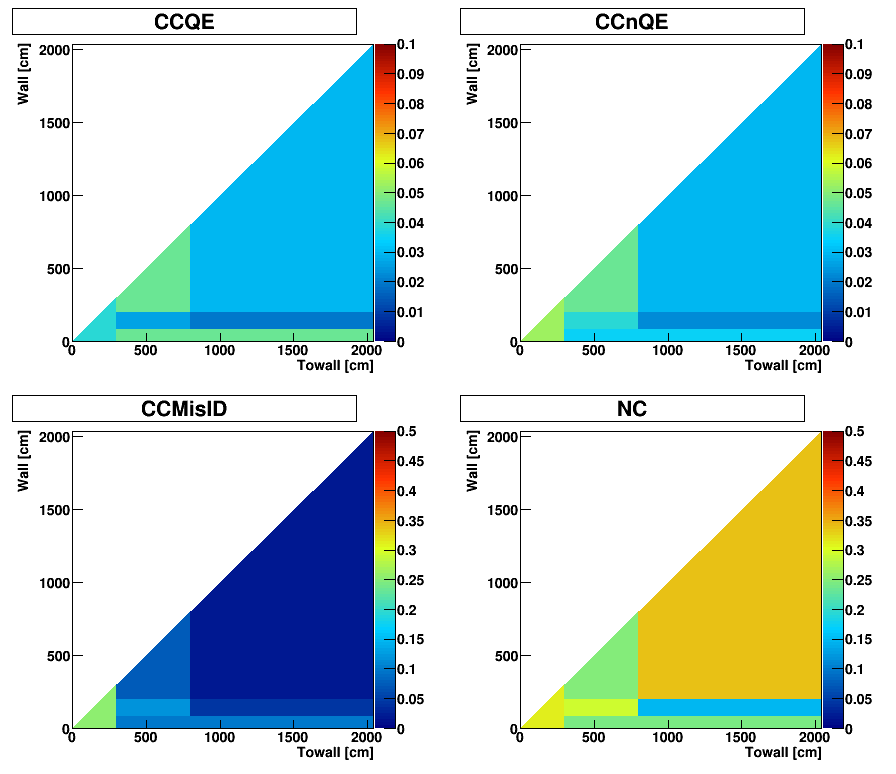
\includegraphics[width=0.6\textwidth]{fv_unc_nue}
  \end{center}
  \caption{Total fractional detector systematic uncertainty in each detector region for selected
  T2K \nue CCQE events.}
  \label{fig:fverrnue}
\end{figure}

\begin{figure}[h]
  \begin{center}
    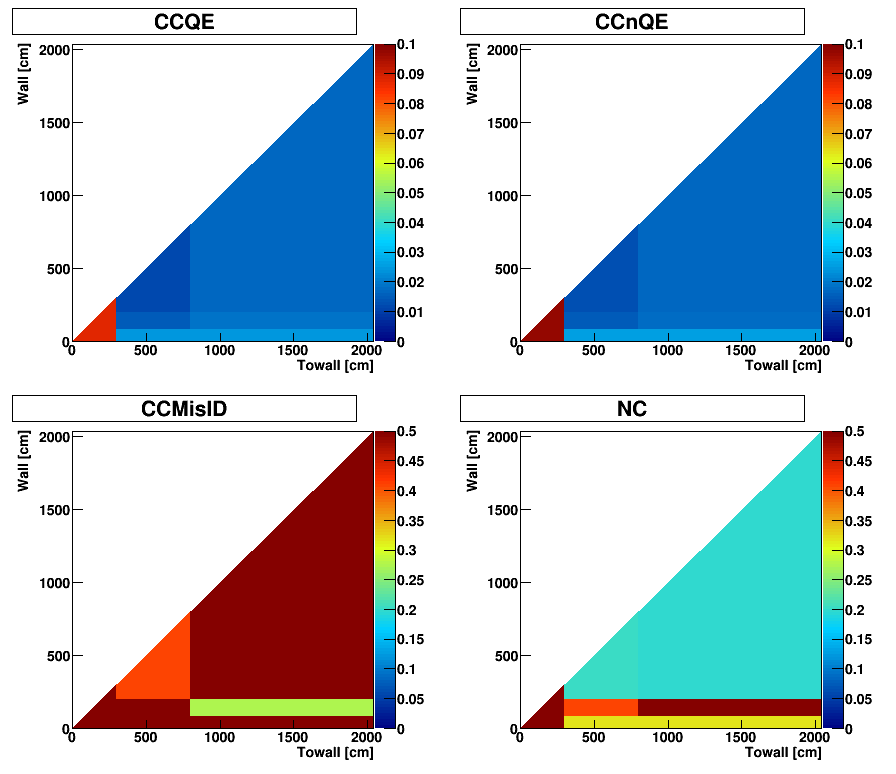
\includegraphics[width=0.6\textwidth]{fv_unc_numu}
  \end{center}
  \caption{Total fractional detector systematic uncertainty in each detector region for selected
  T2K \numu CCQE events.}
  \label{fig:fverrnumu}
\end{figure}

\begin{figure}[h]
  \begin{center}
    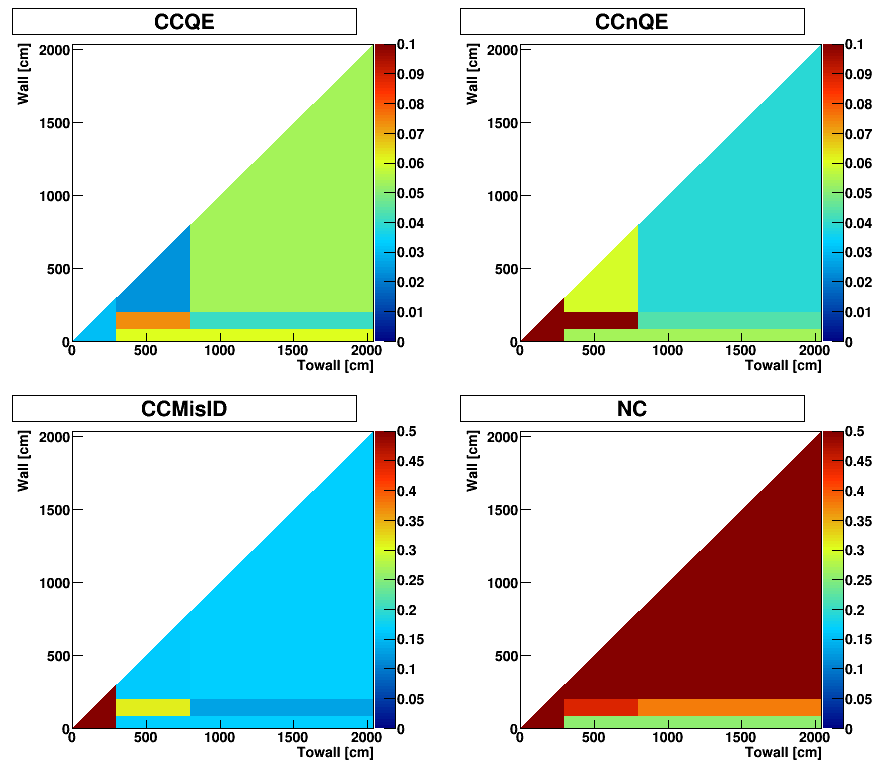
\includegraphics[width=0.6\textwidth]{fv_unc_nue1rpi}
  \end{center}
  \caption{Total fractional detector systematic uncertainty in each detector region for selected
  T2K \nue CC1R$\pi$ events.}
  \label{fig:fverrnue1rpi}
\end{figure}

\begin{table}[h!]
  \centering
  \begin{tabular}{| c | c | c | c | c | c |}
    \hline\hline
    %T2K Sample & Detector Region & CCQE & CCnQE & CCMisID & NC\\
    T2K Sample & Detector Region & \multicolumn{4}{|c|}{Fractional Uncertainty [\%] } \\
    \cline{3-6}
     &  & CCQE & CCnQE & CCMisID & NC \\
    \hline
    \multirow{6}{*}{$\nu_{e}$ CCQE}
      & 0 & 3.8 & 5.3 & 25.0 & 31.5  \\ 
      & 1 & 4.7 & 3.4 & 9.8  & 24.1  \\ 
      & 2 & 2.6 & 3.9 & 11.8 & 29.2  \\ 
      & 3 & 1.9 & 2.3 & 4.0  & 14.5  \\ 
      & 4 & 4.6 & 4.7 & 7.45 & 24.6  \\ 
      & 5 & 2.9 & 2.9 & 1.95 & 33.83 \\ 
      \hline
    \multirow{6}{*}{$\nu_{\mu}$ CCQE}
      & 0 & 8.7 & 9.7 & 83.2 & 66.7 \\ 
      & 1 & 2.4 & 2.5 & 69.8 & 31.6 \\ 
      & 2 & 1.4 & 1.5 & 54.6 & 41.0 \\ 
      & 3 & 1.8 & 1.7 & 27.1 & 58.1 \\ 
      & 4 & 1.2 & 1.2 & 41.0 & 20.0 \\ 
      & 5 & 1.7 & 1.6 & 74.9 & 19.7 \\ 
      \hline
    \multirow{6}{*}{$\nu_{e}$ CC1R$\pi$}
      & 0 & 3.0 & 11.2 & 80.4 & 56.2  \\ 
      & 1 & 6.0 & 5.4  & 16.8 & 25.3  \\ 
      & 2 & 7.4 & 18.4 & 31.2 & 44.1  \\ 
      & 3 & 4.0 & 4.3  & 13.4 & 37.8  \\ 
      & 4 & 2.4 & 5.9  & 16.4 & 182.6 \\ 
      & 5 & 5.3 & 3.8  & 16.6 & 232.7 \\ 
    \hline
  \end{tabular}
  \caption{Table of the values of the fractional uncertainties shown in
  Figures~\ref{fig:fverrnue}-~\ref{fig:fverrnue1rpi}.}
  \label{tab:fverrs}
\end{table}



%-----------------------------------------------------------------------------
% Entering Background Uncertainties
%-----------------------------------------------------------------------------
\subsection{Entering Event Uncertainty}
\label{subsec:entering}

One group of events that requires special attention are the entering background
events.  These events are defined as any event that passes
the T2K event selection cuts for a particular sample and has a true \wall
value less than zero, that is, an event where the vertex originates outside of
the ID\@.  Although the outer detector (OD) is designed to veto these events,
some entering backgrounds remain in the T2K samples.  These events mostly
originate in the 55 cm ``dead region'' between the ID and OD optical barriers.
Such events cannot be rejected by the OD, and due to limited reconstruction
resolution they may be reconstructed with a vertex inside the ID\@.  
There are two main systematic uncertainties that we assign to these events:

\begin{enumerate}
  \item A \wall-dependant systemaic uncertainty to account for data/MC differences in 
    how far into the ID the entering events are reconstructed.
  \item An overall normalization uncertatinty that accounts for data/MC
    differences in the absolute number of entering events
\end{enumerate}

The first systematic is estimated by checking the data/MC differences in the
reconstructed \wall distributions for stopping cosmic muons. We see that the
normalized reconstructed \wall distributions have good agreement near the peak
event density, but slightly worse agreement in the tails, with the data tending
to reconstruct more events further away from the ID wall.  To address this, we
impose an uncertainty as a function of reconstructed \wall that rises from
$4\%$ to almost $50\%$ as shown in Figure~\ref{fig:enteringwall}.

The seconds systematic is estimated by extrapolating the density of
fully-contained (FC) T2K events to the un-simulated dead region.  We find the
un-simulated region contributes and additional $10\%$ to the entering
background normalization (see Figure~\ref{fig:unsim}).  To account for
this in the MC, we increase the overall normalization by $10\%$ and apply an
additional conservative $20\%$ systematic uncertainty weight to cover
additional uncertainties such as the OD efficiency very close to the optical barrier
as well as un-simulated PMT mass in the dead region.  The overall result is a
minimum $30\%$ uncertainty in the entering background, which will penalize the
optimization figure of merit if FV cuts are chosen to allow many of these
entering events into the T2K event samples.

\begin{figure}[h!t]
  \begin{center}
    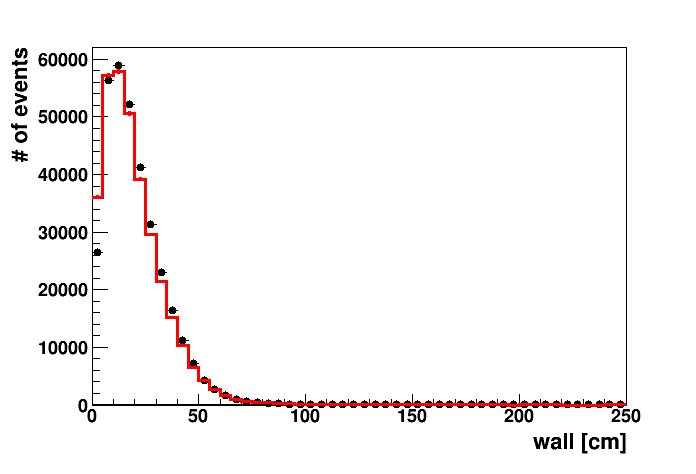
\includegraphics[width=0.4\textwidth]{cosmic_walldist}
    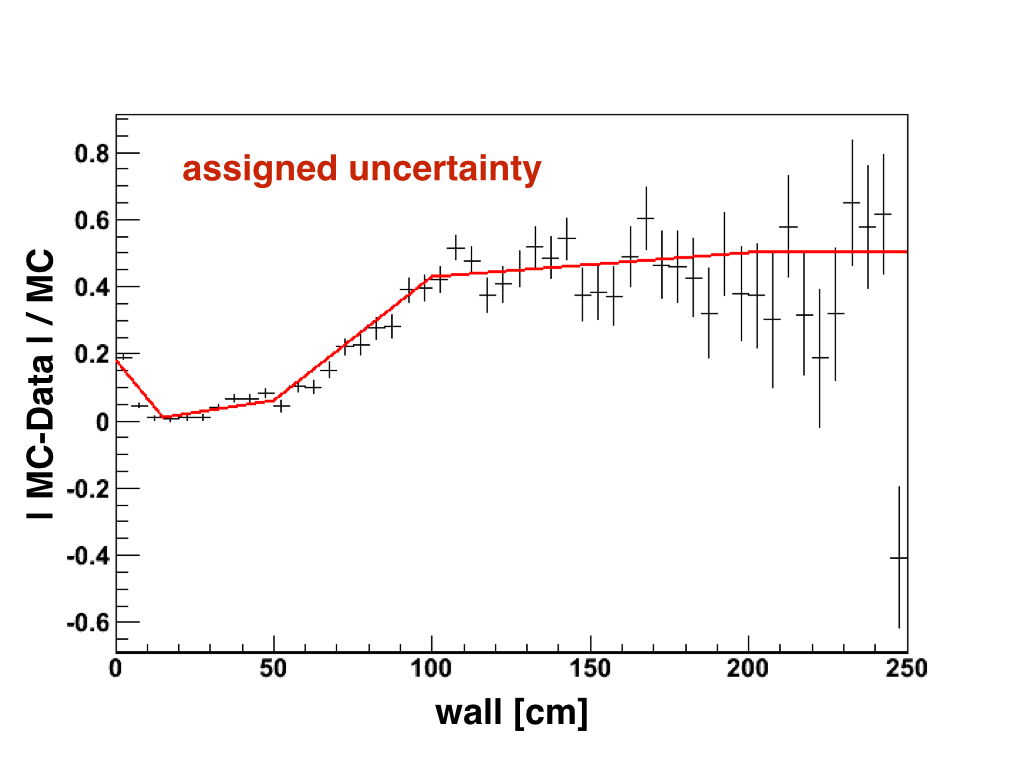
\includegraphics[width=0.4\textwidth]{entering_wall_unc}
  \end{center}
  \caption{Left plot shows the normalized \wall distributions for stopping cosmic muons.  Red histogram
  shows the MC simulation and black points show the data in each bin.  The right plot shows the absolute 
  data/MC fractional difference.  The right plot is used to apply a \wall-dependant systematic uncertainty
  for entering events.}
  \label{fig:enteringwall}
\end{figure}

\begin{figure}[h!t]
  \begin{center}
    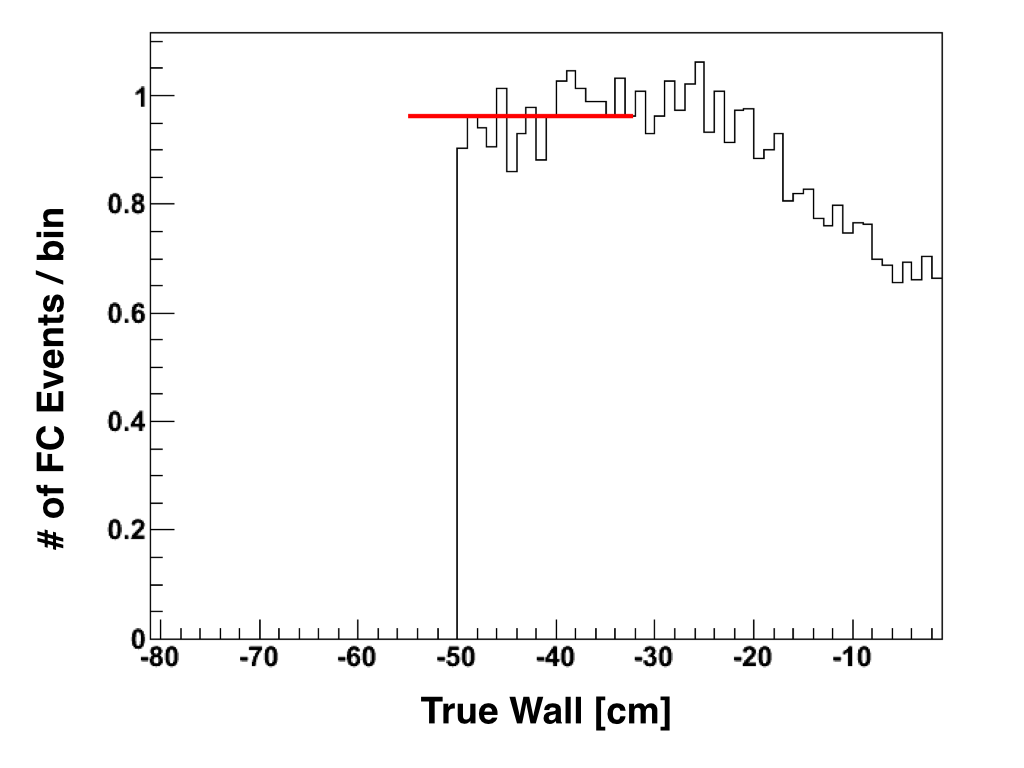
\includegraphics[width=0.4\textwidth]{unsim_region}
    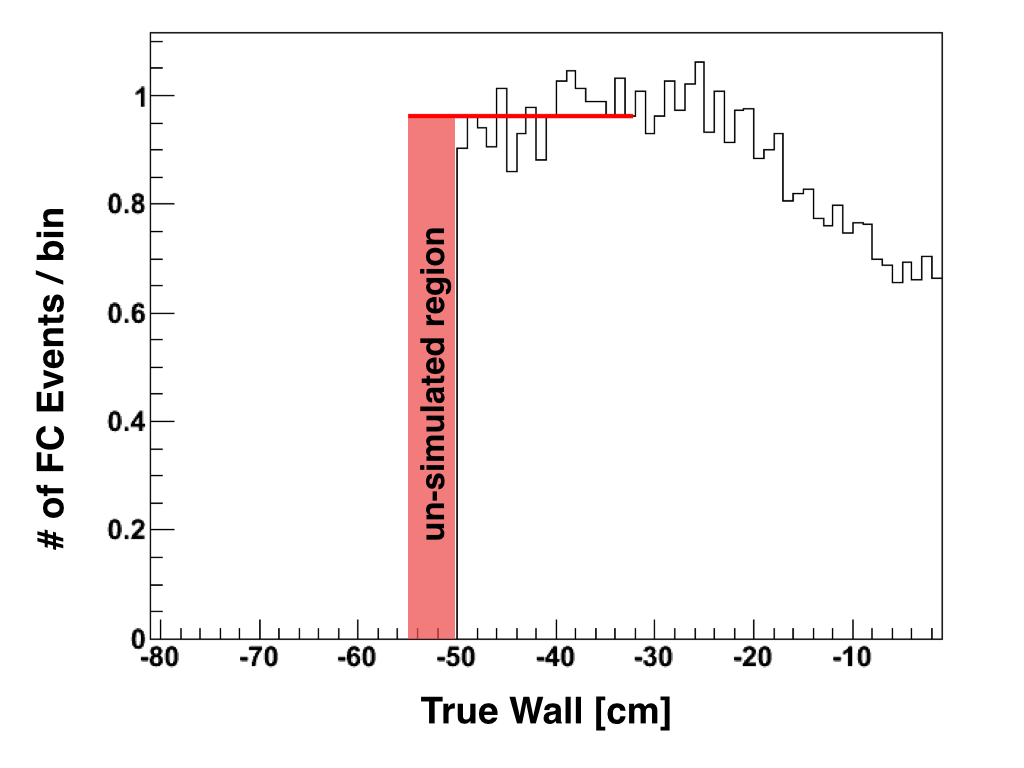
\includegraphics[width=0.4\textwidth]{unsim_region_extrap}
  \end{center}
  \caption{Left plot shows the true MC \wall distribution for entering T2K
  events that are not rejected by the OD activity cuts.  The ID optical
  boundary is at $\wall = 0$ cm.  The OD optical boundary is located at  $\wall
  = -55$ cm. The region between the ID and the OD optical boundaries is the
  so-called ``dead region''.  Only the inner 50 cm of the 55 cm dead region is
  simulated in the MC simulation.  To account for this, the MC distribution is
  extrapolated into the un-simulated region (red line on left plot).  The
  extrapolation is then integrated to estimate the number of un-simulated
  events.  The number of un-simulated events (red area on right plot) is 10\%
  of the total number of entering events. This 10\% normalization increase is
  accounted for when optimizing the detector fiducial volume.}
  \label{fig:unsim}
\end{figure}

%\begin{figure}[h!t]
%  \begin{center}
%    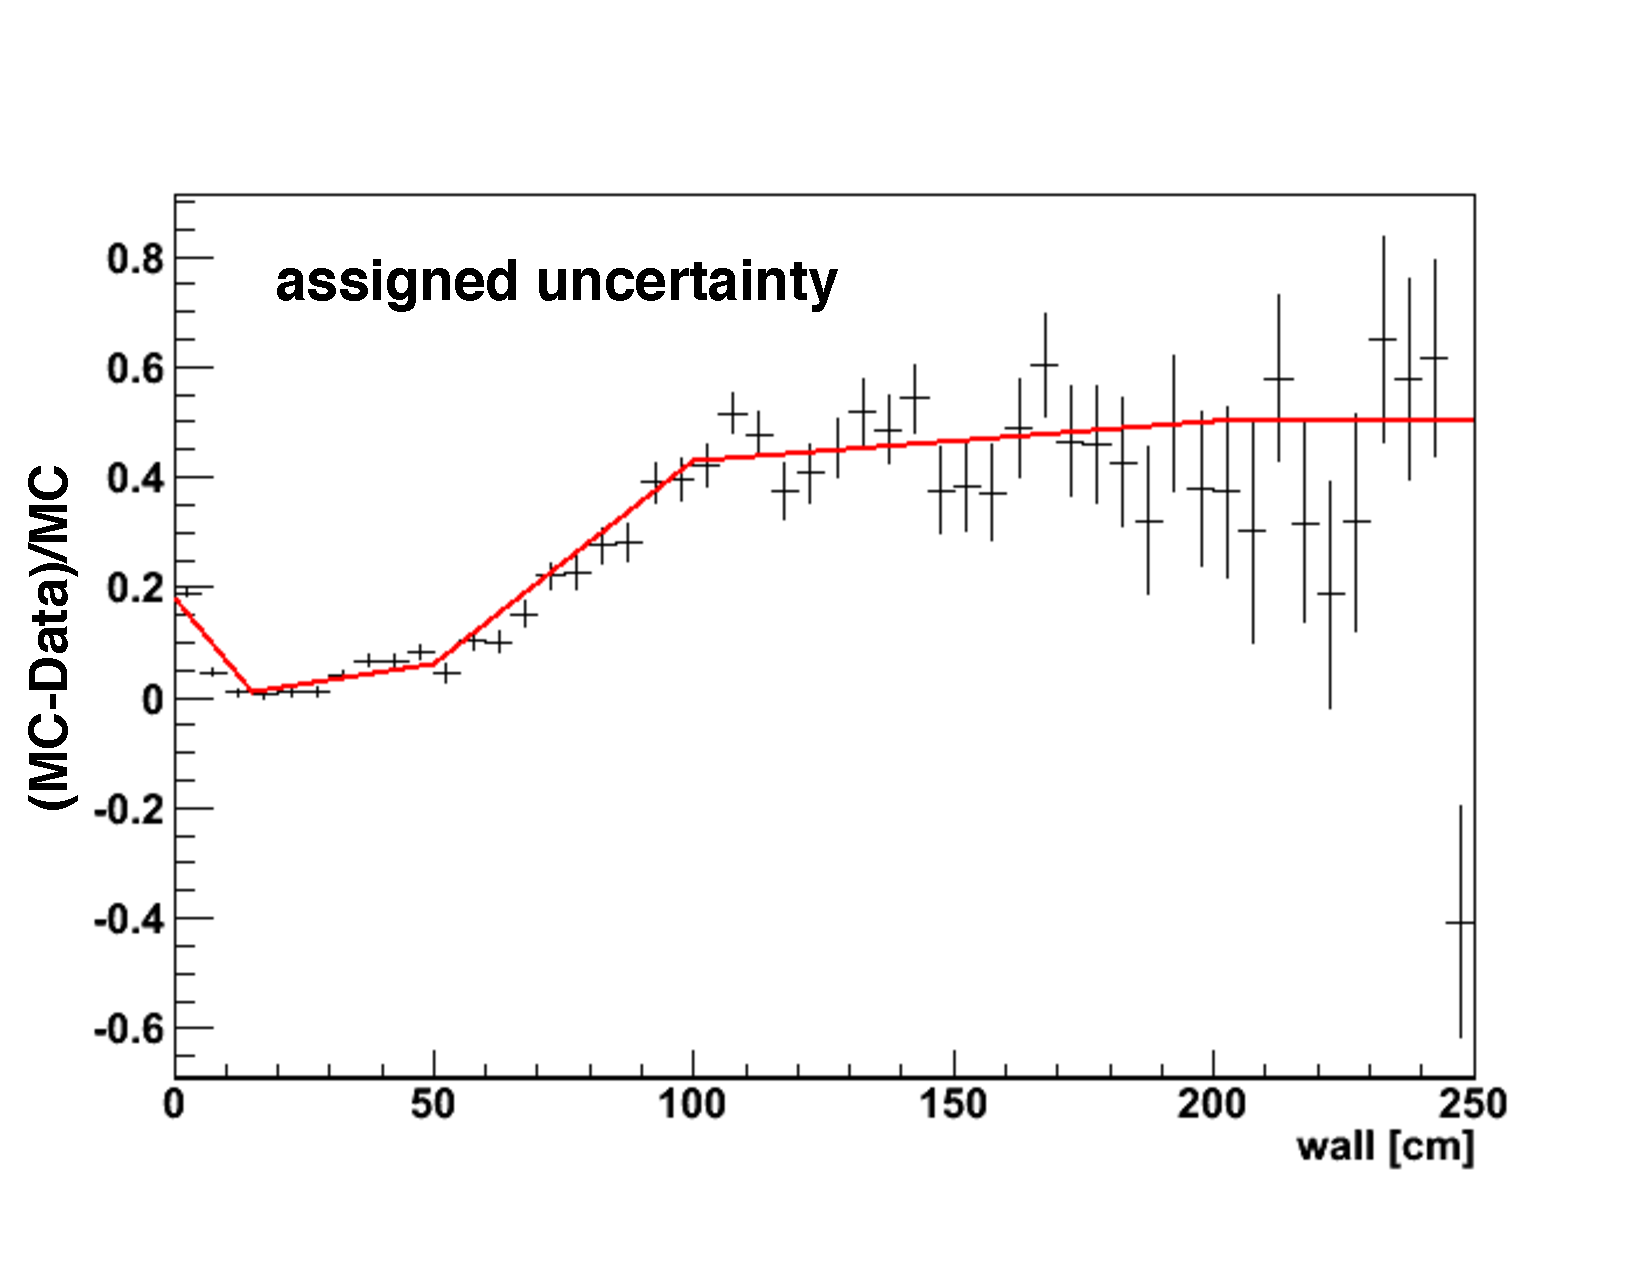
\includegraphics[width=0.4\textwidth]{entering_unc}
%    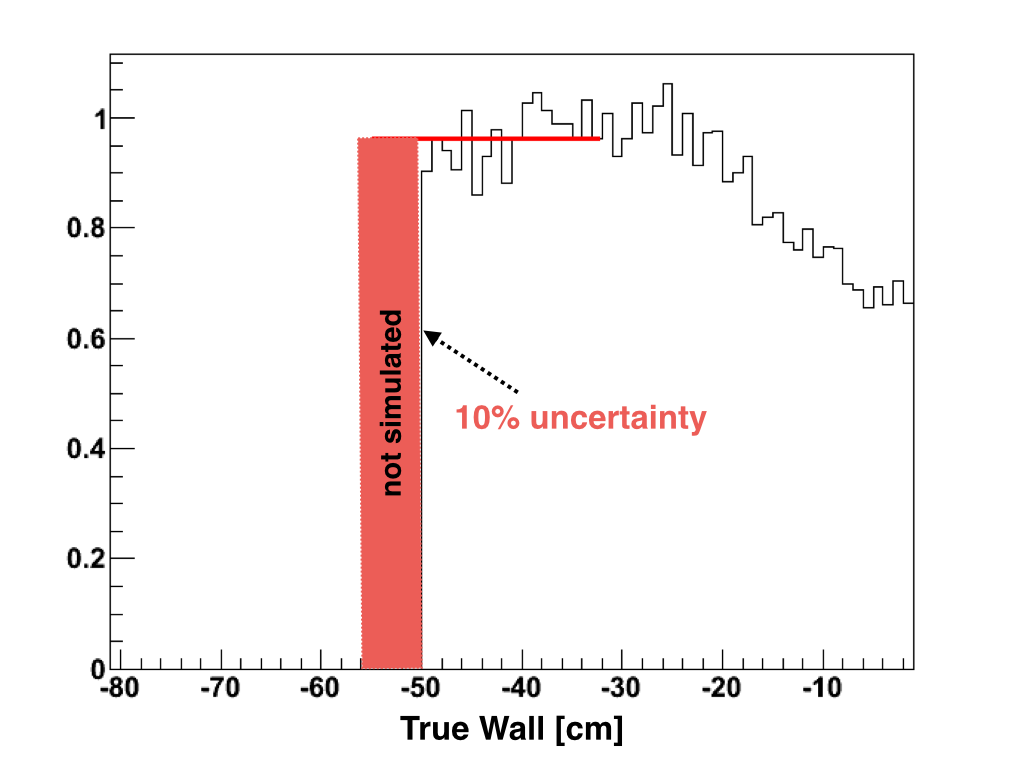
\includegraphics[width=0.4\textwidth]{entering_norm}
%  \end{center}
%  \caption{Left plot shows the \wall-dependant systematic applied to account
%  for data/MC differences in how far into the ID entering backgrounds are
%  reconstructed.  Right plot shows the overall normalization increase applied
%  to all entering events from un-simulated dead region volume.}
%  \label{fig:enteringerr}
%\end{figure}






%-----------------------------------------------------------------------------
% FV Cut Floors
%-----------------------------------------------------------------------------
\subsection{Minimum FV Cut Constraints}
\label{subsec:floor}


Before determining the optimal FV cuts, it is important to first consider the
limits of the FV optimization framework and determine the extent to which we
can apply the results.  The figure of merit described in Equation~\ref{eq:fom}
essentially models the contributions to the sensitivity coming from the overall
statistical size, overall purity, and overall uncertainty.  In this simplified
model, the effect of the neutrino energy resolution is not explicitly included.
We should therefore be careful to avoid introducing events with poor energy
resolution into our T2K samples, since they may have a negative impact on the
sensitivity that is not accounted for in this simple model. 

Studies of the fiTQun energy resolution show that the energy reconstruction
performance appears stable in detector regions with $towall \ge 150$ cm and
$wall \ge 50$ cm, and in the regions below these values fiTQun tends to reconstruct 
a systematically smaller neutrino energy (see Figure~\ref{fig:erec}).  To omit these regions we
choose to optimize the figure of merit subject to the constraint that $towall
\ge 150$ cm and $wall \ge 50$ cm.  This effectively puts a ``floor'' on the
values of the optimized fiTQun FV cuts.

\begin{figure}[h!]
  \begin{center}
    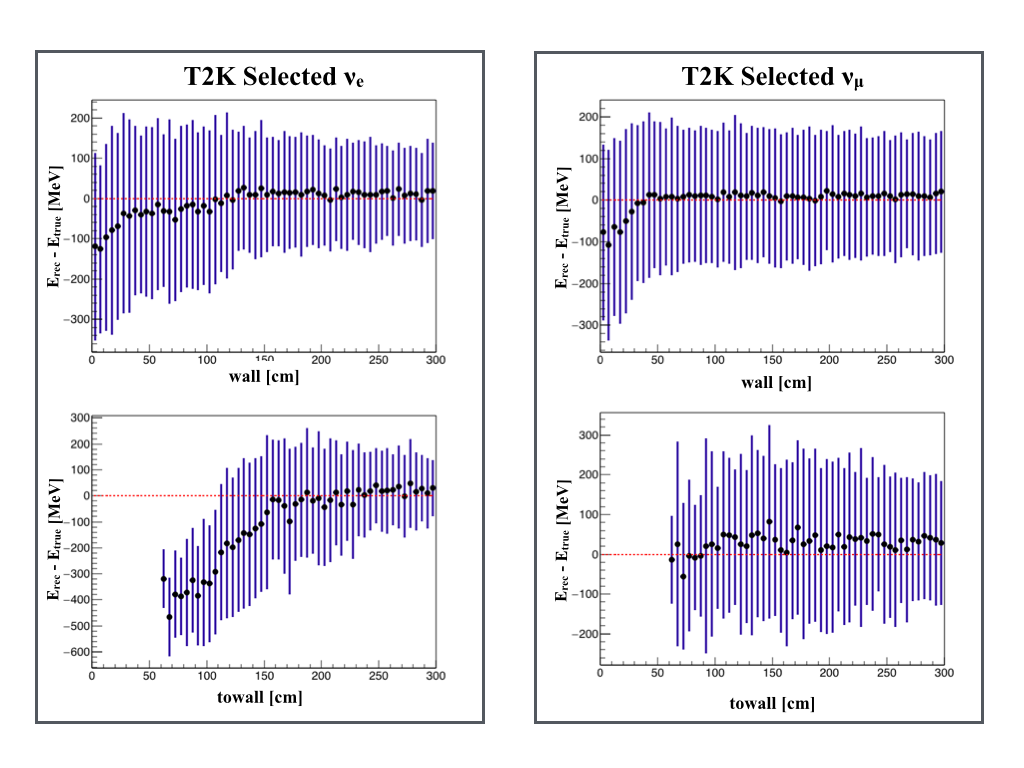
\includegraphics[width=0.7\textwidth]{erec_walltowall}
  \end{center}
  \caption{Neutrino energy residuals for both the \nue and \numu fiTQun event selections in bins
  of \wall and \towall.  The contents of each bin shows the average deviation of the reconstructed
  neutrino energy from the true neutrino energy in a particular \towall or 
  \wall region.  The error bar shows the RMS of the distribution of residual values.}
  \label{fig:erec}
\end{figure}

Although the bias in neutrino energy reconstruction is the main reason for
imposing these FV cut floors, the cut floors also make this analysis less
sensitive to some potential systematics that are difficult to quantify, such
as:
%
\begin{itemize}
  \item Un-simulated PMT structure near the ID wall and in the so-called ``dead region'' between the ID and the OD.
  \item Un-simulated ``dead region'' volume.
  \item Effect of PMTs protruding into the SK ID volume.
  \item Assumption of a smoothly cylindrical detector geometry in the MC
    simulation, as opposed to the actual SK geometry consisting of multiple
    flat panels.
\end{itemize}
%
The cut floors may be removed for future FV cut optimization analyses if the
above systematics, as well as the energy reconstruction bias, are understood and
incorporated into the figure of merit. 



%-----------------------------------------------------------------------------
% FV Optimization Results
%-----------------------------------------------------------------------------
\subsection{FV Optimization Results}
\label{subsec:fvresults}


With the region-dependant detector systematics estimated from the atmospheric MC fit as described in Section~\ref{subsec:fvunc},
we are now finally in a position to evaluate the figure of merit described in Equation~\ref{eq:fom}.  For every T2K MC event,
we can assign a total systematic uncertainty weight according to: 
%
\begin{equation}
  w_{syst} = w_{detector} + w_{xsec} + w_{entering}
\end{equation}
%
Where $w_{detector}$ is a detector-region dependant uncertainty taken from the
fractional uncertainty defined in Section~\ref{subsec:fvunc}, $w_{xsec}$ is
taken from the uncertainties shown in Table~\ref{tab:alpha}, and $w_{entering}$
is an additional systematic weight applied only to entering events as described
in Section~\ref{subsec:entering}.  The sum of the systematic weights for each
T2K sample is used to calculate $\sigma^{2}_{syst}$ in Equation~\ref{eq:fom}
for a possible set of FV cuts. The overall procedure for optimizing the FV cuts
can be outlined as follows:
%
\begin{enumerate}
  \item Choose a particular $(towall,wall)$ FV cut point
  \item Loop over all of the T2K MC events and calculate $\frac{\partial
    \hat{N}}{\partial \theta}$ and $\sigma^{2}_{syst}$ as oulined in the
    previous sections.
  \item Evaluate the figure of merit by calculating Equation~\ref{eq:fom}.
  \item Return to Step 1 and repeat for a new $(towall,wall)$ cut point.
  \item After sampling many $(towall,wall)$ in some range, choose the point
    that maximizes the figure of merit subject to the constraint that $wall \ge
    50 cm$.
\end{enumerate}
%
The plots of the figure of merit for each of the T2K data samples are shown in
Figure~\ref{fig:fom}.  For both the \numu and the \nue CC1R $\pi$ samples, the
maximum of the figure of merit has a \wall cut that lies outside of
the predetermined FV cut floor.  In these cases, we fix $wall = 50$ cm and
choose the \towall cut that maximizes the figure of merit.  The final optimized
FV cut values for the fiTQun T2K selections are listed in
Table~\ref{tab:fvcuts}.

\begin{table}
  \centering
  \begin{tabular}{c|c|c}
    \hline\hline
    T2K Sample & Towall Cut [cm] & Wall Cut [cm] \\
    \hline
    \nue CCQE & 170 & 80 \\
    \numu CCQE & 250 & 50 \\
    \nue CC1R$\pi$ & 270 & 50 \\
    \hline
  \end{tabular}
  \caption{Optimized fiTQun FV cuts for the T2K analysis.}
  \label{tab:fvcuts}
\end{table}

\begin{figure}[h]
  \begin{center}
    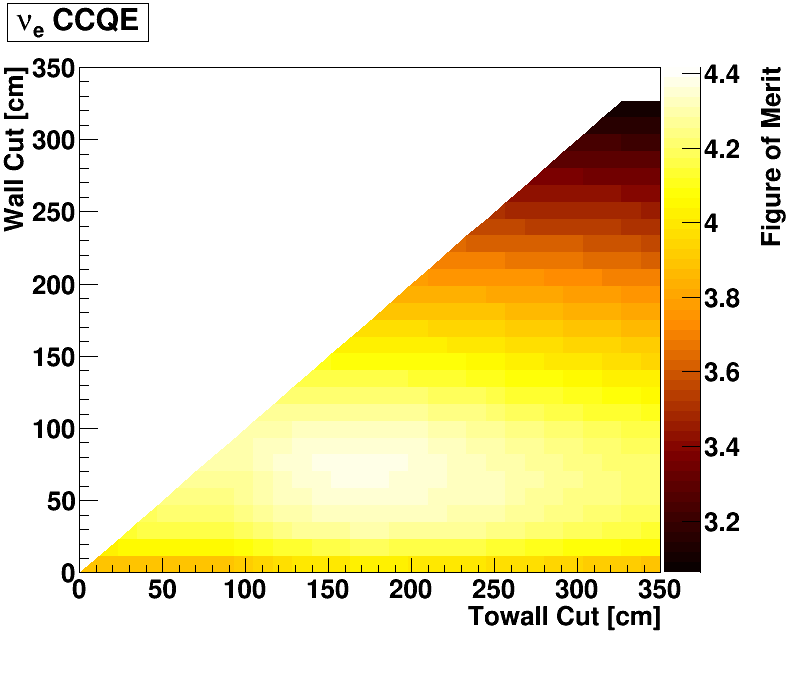
\includegraphics[width=0.45\textwidth]{hfom_nue}
    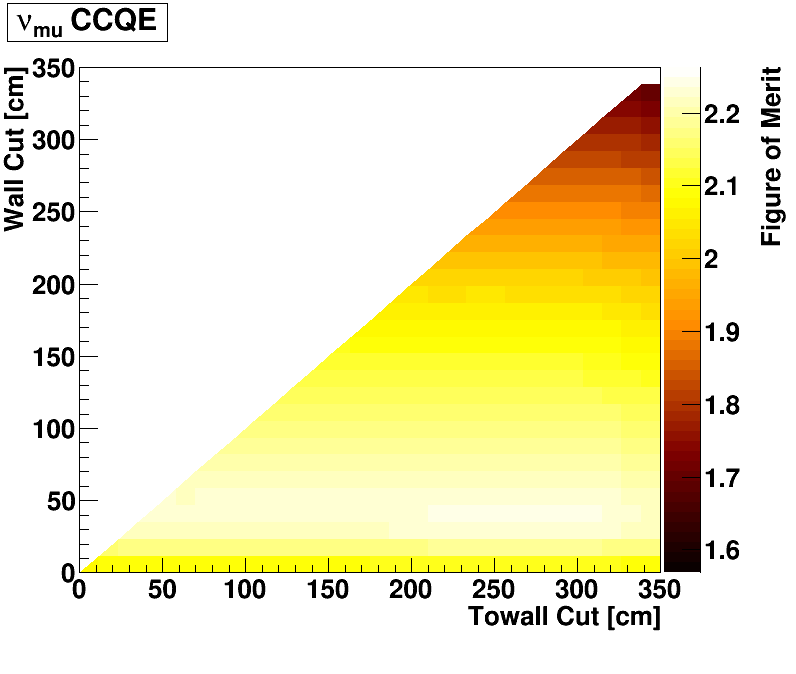
\includegraphics[width=0.45\textwidth]{hfom_numu}
    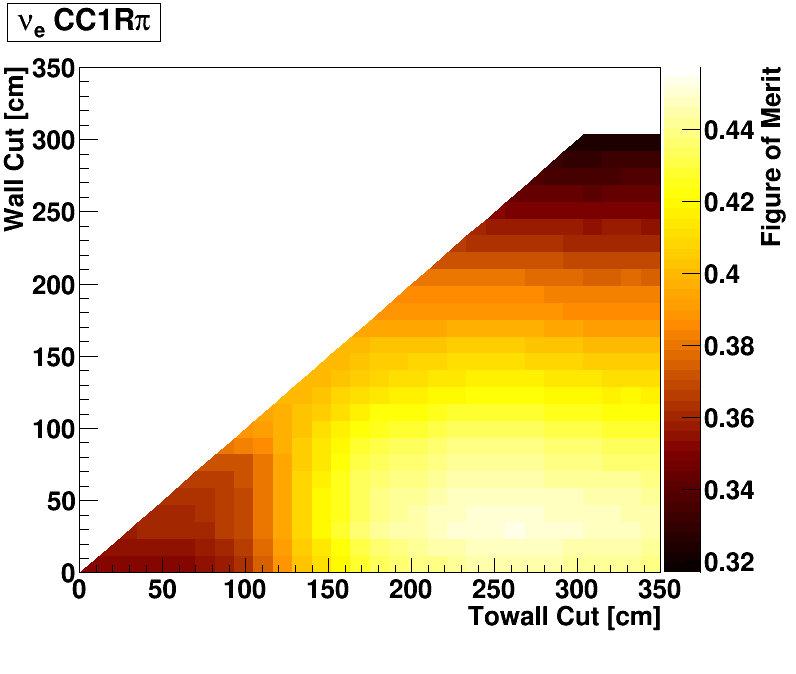
\includegraphics[width=0.45\textwidth]{hfom_nuecc1rpi}
  \end{center}
  \caption{Plots of the figure of merit for FV cut optimization at various
  $(towall,wall)$ points for each of the T2K event selections. The maximum value of the figure of merit with the
  constraint $\wall \geq 50 cm$ is used to determine the fiTQun FV cuts listed in
  Table~\ref{tab:fvcuts}}
  \label{fig:fom}
\end{figure}



%-----------------------------------------------------------------------------
% Discusstion of Results
%-----------------------------------------------------------------------------
\subsection{Discussion of fiTQun FV Cuts}
\label{subsec:fvdiscuss}

The factors that drive the FV cut results of Section~\ref{subsec:fvresults} can
be largely understood by examining the distributions of various signal
and background channels in \wall and \towall for each of the T2K event
selections.  These figures are shown for each T2K sample in Section~\ref{sec:evtdist}.
The optimization figure of merit (Equation~\ref{eq:fom}) is
penalized heavily when backgrounds (any NC, mis-identified, or entering event)
are allowed into the sample.  This is due to the fact that such events are
defined to not contribute to the numerator in the figure of merit, and they
contribute to both the statistical and systematic uncertainty in the
denominator. Since the systematics are generally larger in the
small \wall and small \towall regions, the figure of merit will naturally
disfavor cuts that add significant backgrounds from these regions.  

Examination of the selected \nue events in bins of \towall shows a clear
increase in background events in the small \towall and small \wall regions.
The small \towall region in particular features a sharp peak in the
mis-identified muon background.  This feature should be expected, since small
\towall events may have a smaller projected Cherenkov ring which makes
discrimination between electrons and muons more difficult, and also the decay
electron ring may be completely lost. It is this peak in the background that pushes
the optimal FV cuts away from the small \towall region.  It should be noted,
however, that although the mis-IDed background is very dense in the small
\towall region, the integrated size is only about one event, so the overall
contribution to the selected \nue T2K sample is not so large, and the peak
is almost completely rejected by the optimized FV cuts.

For the selected \nue events in small \wall regions, we again see a peak in the
background events.  In this case, the important backgrounds are the entering and
NC events. The entering events are concentrated in the $wall < 50 cm$ region,
whereas the NC events have a broader peak that results in somewhat tighter cut
on \wall compared to the other T2K samples.

The distributions of the selected T2K \nue CC1R$\pi$ events show peaks in the
background events that are generally similar to the selected \nue events.  Some
important differences are a much larger peak in the mis-ID background (coming
presumably from the loosened decay electron cut), and a smaller NC background
peak.  This results in a tighter \towall cut to reject the muon background, but
a looser \wall cut since the NC background is less problematic.

For the selected \numu events, the signal and background distributions are
noticeably different.  The key difference in this case is that there is no
sharp peak in the background events at small \towall values.  This combined
with the fact that there is a slow tapering off in the density of selected
\numu events at small \towall results in a very loose constraint on the optimal
\towall cut.  This can be seen in the plots of the figure of merit shown in
Figure~\ref{fig:fom}.  In the absence of large peaks in the backgrounds, the
\numu \towall cut is determined by the systematic uncertainty on the signal in
the small \towall regions.  Since these uncertainties are generally less
constrained in the small \towall regions due to lack of statistics, the optimization disfavors
the small \towall region as well.

It is interesting to note that although none of the FV cuts were tuned ``by
hand'' by explicitly checking the \towall and \wall distributions, the
optimized cuts for each sample manage to avoid regions with very large and/or
very uncertain backgrounds.  This seems to imply that the figure of merit
expressed in Equation~\ref{eq:fom} provides a fairly robust way of quantifying
the trade-offs between statistics, purity, and uncertainty.  Additional
information about the event composition for each T2K sample can be found in
TN-319~\cite{tn319}.

\FloatBarrier

%%% NUE %%%%%%%%%%%%%%%%%%%%%%%%%%%%%%%%%%%%%%%%%%%%%%%%
%\begin{figure}[h]
%  \begin{center}
%    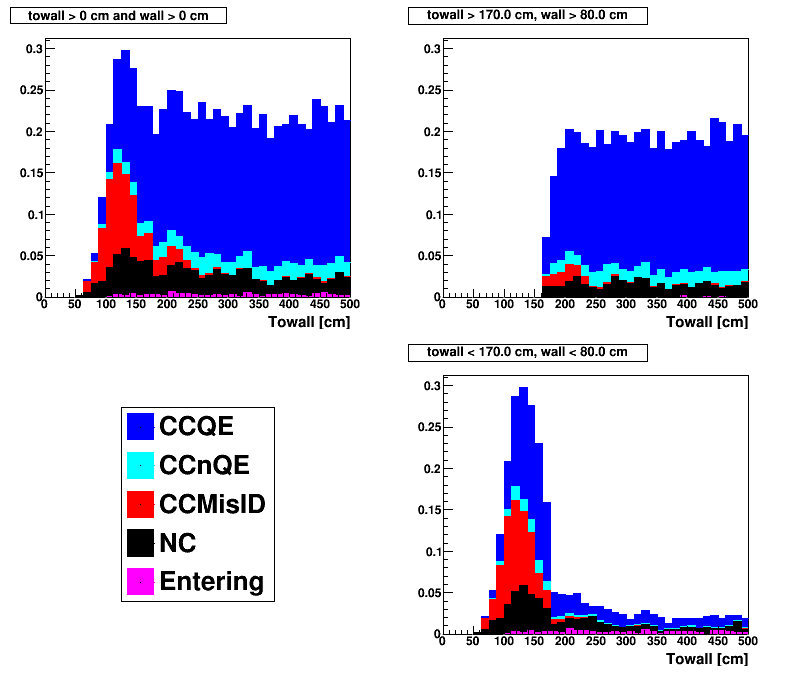
\includegraphics[width=0.9\textwidth]{tw170_nue__towall_}
%  \end{center}
%  \caption{Plots of the various MC categories that pass the T2K \nue
%  topological cuts binned in \towall in various detector regions. Upper left
%  plot shows the distribution for only fully-contained cuts (i.e. FV cut is \@ $wall > 0$ cm).
%  Upper right plot shows the distribution for the optimized FV cut for this selction.
%  Lower Right plot shows the distribution of the events \emph{rejected} by the optimized
%  FV cuts for this sample.
%  }
%  \label{fig:compnuetowall}
%\end{figure}
%
%
%\begin{figure}[h]
%  \begin{center}
%    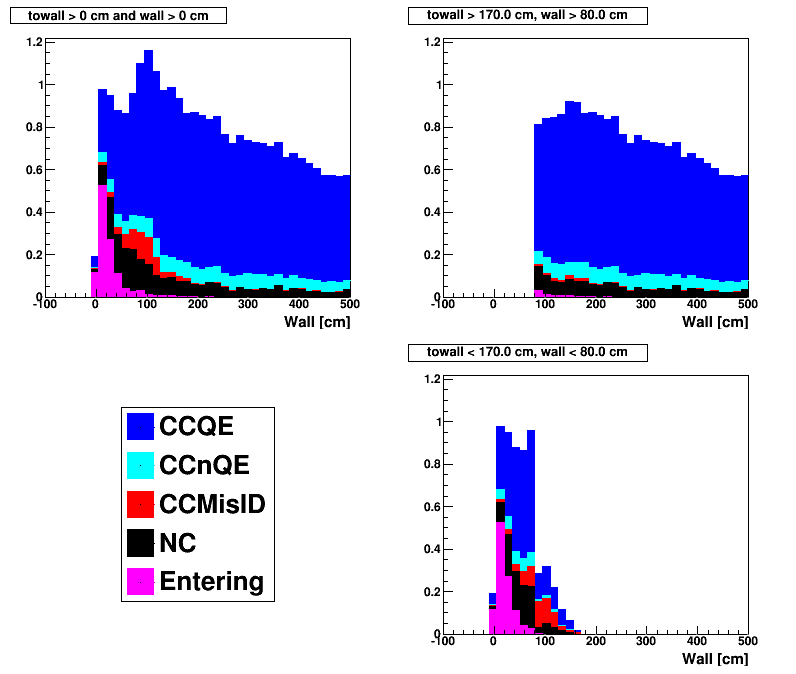
\includegraphics[width=0.9\textwidth]{tw170_nue__wall_}
%  \end{center}
%  \caption{Plots of the various MC categories that pass the T2K \nue
%  topological cuts binned in \wall in various detector regions. Upper left
%  plot shows the distribution for only fully-contained cuts (i.e. FV cut is \@ $wall > 0$ cm).
%  Upper right plot shows the distribution for the optimized FV cut for this selction.
%  Lower Right plot shows the distribution of the events \emph{rejected} by the optimized
%  FV cuts for this sample.
%  }
%  \label{fig:compnuewall}
%\end{figure}
%
%
%\begin{figure}[h]
%  \begin{center}
%    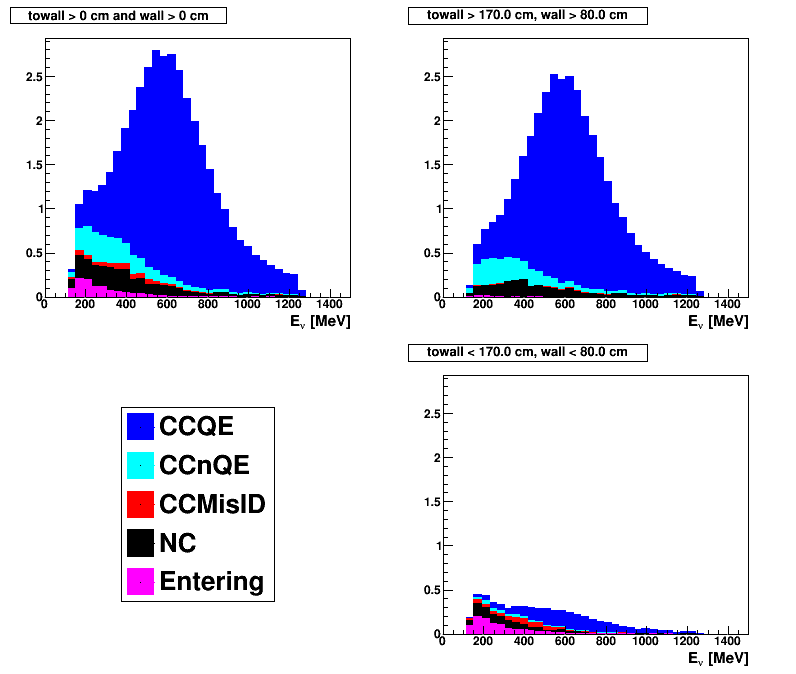
\includegraphics[width=0.9\textwidth]{tw170_nue__erec_}
%  \end{center}
%  \caption{Plots of the various MC categories that pass the T2K \nue
%  topological cuts binned in reconstructed neutrino energy in various detector
%  regions. Upper left plot shows the distribution for only fully-contained cuts
%  (i.e. FV cut is \@ $wall > 0$ cm).  Upper right plot shows the distribution
%  for the optimized FV cut for this selction.  Lower Right plot shows the
%  distribution of the events \emph{rejected} by the optimized FV cuts for this
%  sample.
%  }
%  \label{fig:compnueerec}
%\end{figure}
%
%%% NUMU %%%%%%%%%%%%%%%%%%%%%%%%%%%%%%%%%%%%%%%%%%%%%%%%
%\begin{figure}[h]
%  \begin{center}
%    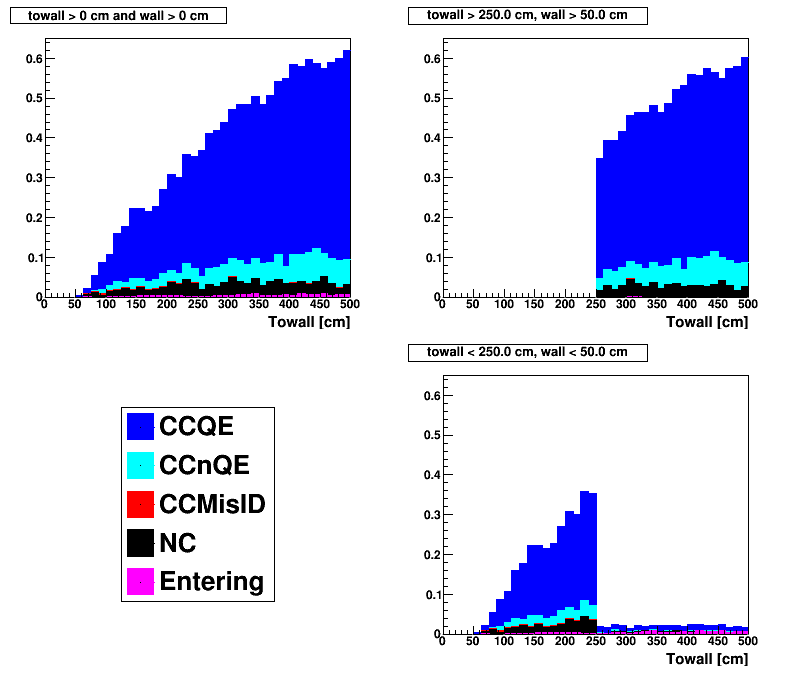
\includegraphics[width=0.9\textwidth]{tw250_numu__towall_}
%  \end{center}
%  \caption{Plots of the various MC categories that pass the T2K \numu
%  topological cuts binned in \towall in various detector regions. Upper left
%  plot shows the distribution for only fully-contained cuts (i.e. FV cut is \@ $wall > 0$ cm).
%  Upper right plot shows the distribution for the optimized FV cut for this selction.
%  Lower Right plot shows the distribution of the events \emph{rejected} by the optimized
%  FV cuts for this sample.
%  }
%  \label{fig:compnumutowall}
%\end{figure}
%
%
%\begin{figure}[h]
%  \begin{center}
%    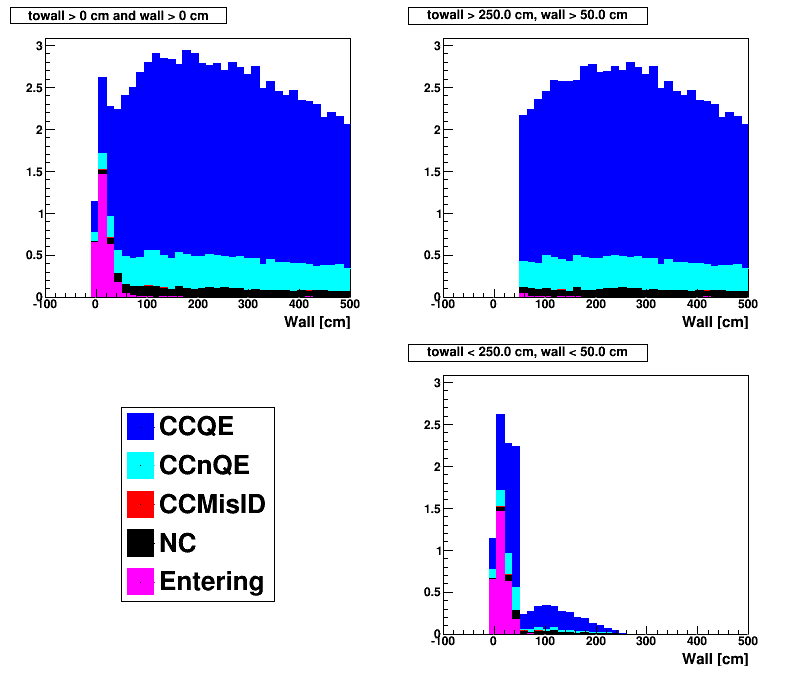
\includegraphics[width=0.9\textwidth]{tw250_numu__wall_}
%  \end{center}
%  \caption{Plots of the various MC categories that pass the T2K \numu
%  topological cuts binned in \wall in various detector regions. Upper left
%  plot shows the distribution for only fully-contained cuts (i.e. FV cut is \@ $wall > 0$ cm).
%  Upper right plot shows the distribution for the optimized FV cut for this selction.
%  Lower Right plot shows the distribution of the events \emph{rejected} by the optimized
%  FV cuts for this sample.
%  }
%  \label{fig:compnumuwall}
%\end{figure}
%
%
%\begin{figure}[h]
%  \begin{center}
%    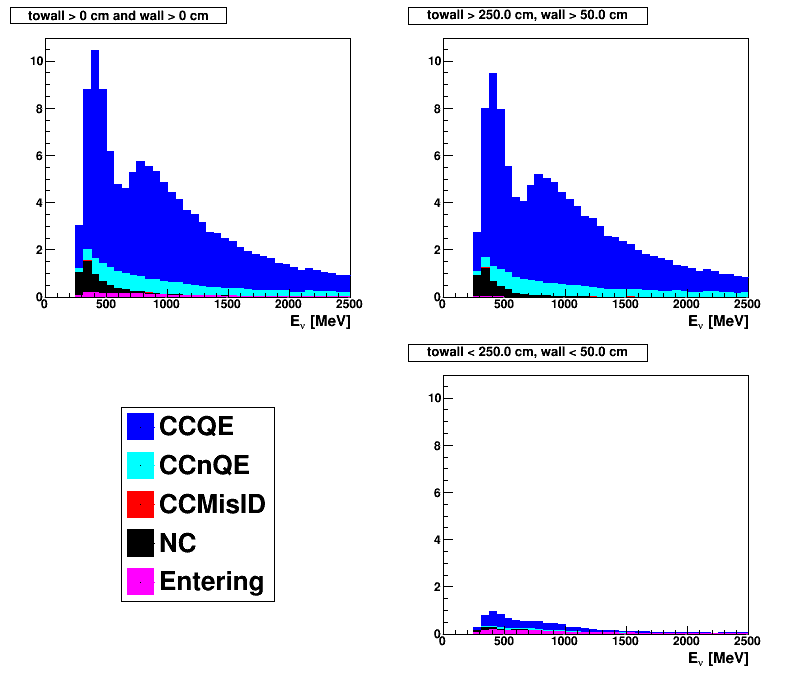
\includegraphics[width=0.9\textwidth]{tw250_numu__erec_}
%  \end{center}
%  \caption{Plots of the various MC categories that pass the T2K \numu
%  topological cuts binned in reconstructed neutrino energy in various detector
%  regions. Upper left plot shows the distribution for only fully-contained cuts
%  (i.e. FV cut is \@ $wall > 0$ cm).  Upper right plot shows the distribution
%  for the optimized FV cut for this selction.  Lower Right plot shows the
%  distribution of the events \emph{rejected} by the optimized FV cuts for this
%  sample.
%  }
%  \label{fig:compnumuerec}
%\end{figure}
%
%
%%% NUE1RPI %%%%%%%%%%%%%%%%%%%%%%%%%%%%%%%%%%%%%%%%%%%%%%%%
%\begin{figure}[h]
%  \begin{center}
%    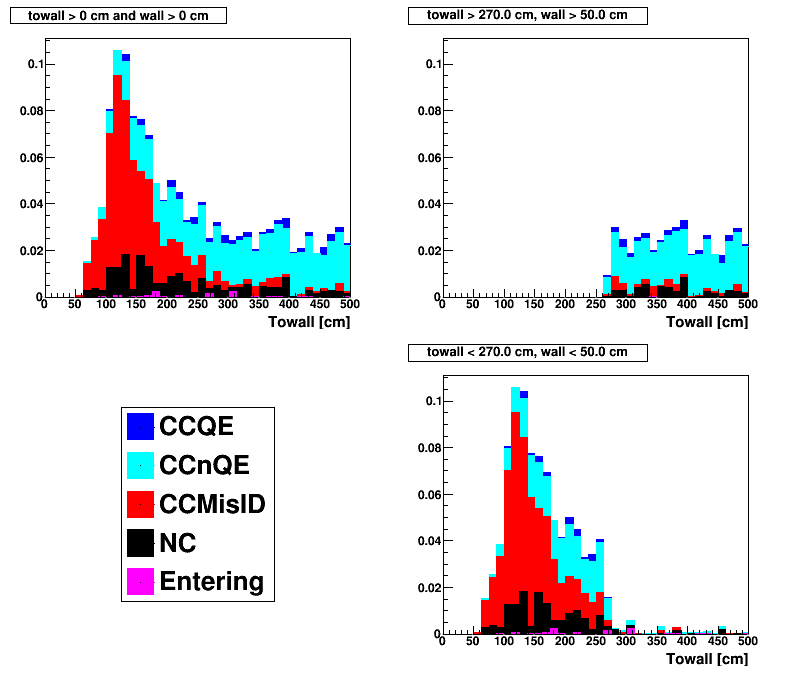
\includegraphics[width=0.9\textwidth]{tw270_nue1rpi__towall_}
%  \end{center}
%  \caption{Plots of the various MC categories that pass the T2K  \nue CC1R$pi$
%  topological cuts binned in \towall in various detector regions. Upper left
%  plot shows the distribution for only fully-contained cuts (i.e. FV cut is \@ $wall > 0$ cm).
%  Upper right plot shows the distribution for the optimized FV cut for this selction.
%  Lower Right plot shows the distribution of the events \emph{rejected} by the optimized
%  FV cuts for this sample.
%  }
%  \label{fig:compnue1rpitowall}
%\end{figure}
%
%
%\begin{figure}[h]
%  \begin{center}
%    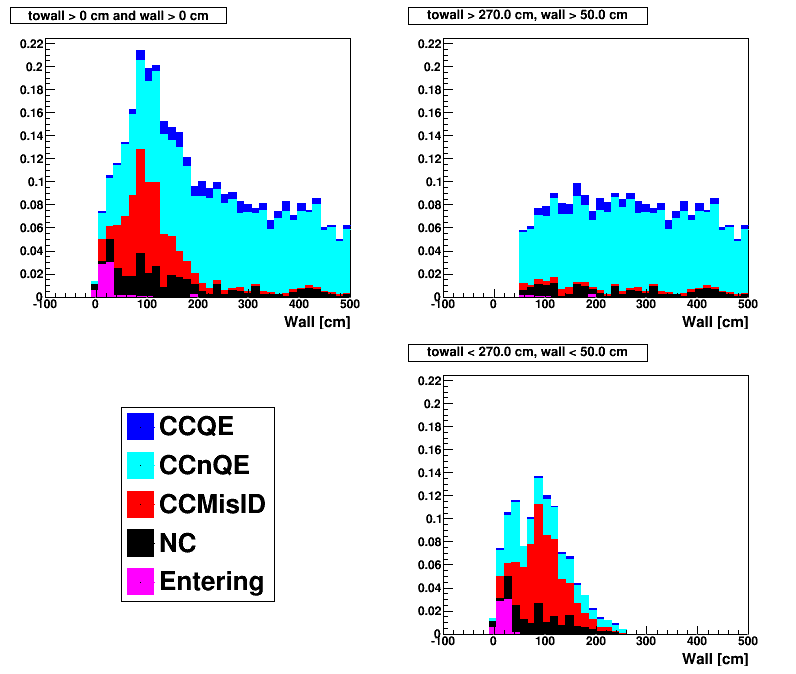
\includegraphics[width=0.9\textwidth]{tw270_nue1rpi__wall_}
%  \end{center}
%  \caption{Plots of the various MC categories that pass the T2K \nue CC1R$pi$
%  topological cuts binned in \wall in various detector regions. Upper left plot
%  shows the distribution for only fully-contained cuts (i.e. FV cut is \@ $wall
%  > 0$ cm).  Upper right plot shows the distribution for the optimized FV cut
%  for this selction.  Lower Right plot shows the distribution of the events
%  \emph{rejected} by the optimized FV cuts for this sample.
%  }
%  \label{fig:compnue1rpiwall}
%\end{figure}
%
%
%\begin{figure}[h]
%  \begin{center}
%    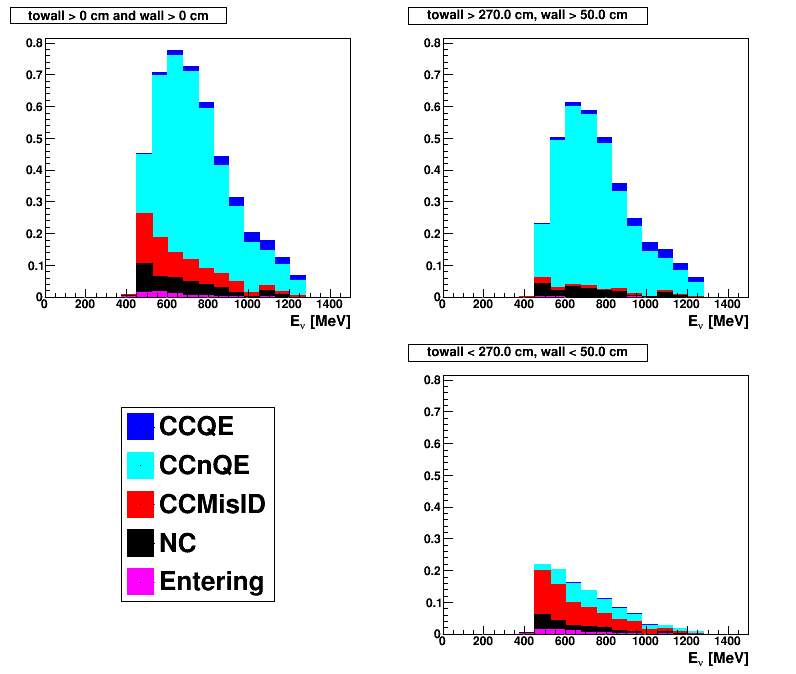
\includegraphics[width=0.9\textwidth]{tw270_nue1rpi__erec_}
%  \end{center}
%  \caption{Plots of the various MC categories that pass the T2K \nue CC1R$pi$
%  topological cuts binned in reconstructed neutrino energy in various detector
%  regions. Upper left plot shows the distribution for only fully-contained cuts
%  (i.e. FV cut is \@ $wall > 0$ cm).  Upper right plot shows the distribution
%  for the optimized FV cut for this selction.  Lower Right plot shows the
%  distribution of the events \emph{rejected} by the optimized FV cuts for this
%  sample.
%  }
%  \label{fig:compnue1rpierec}
%\end{figure}

%\begin{figure}[h]
%  \begin{center}
%    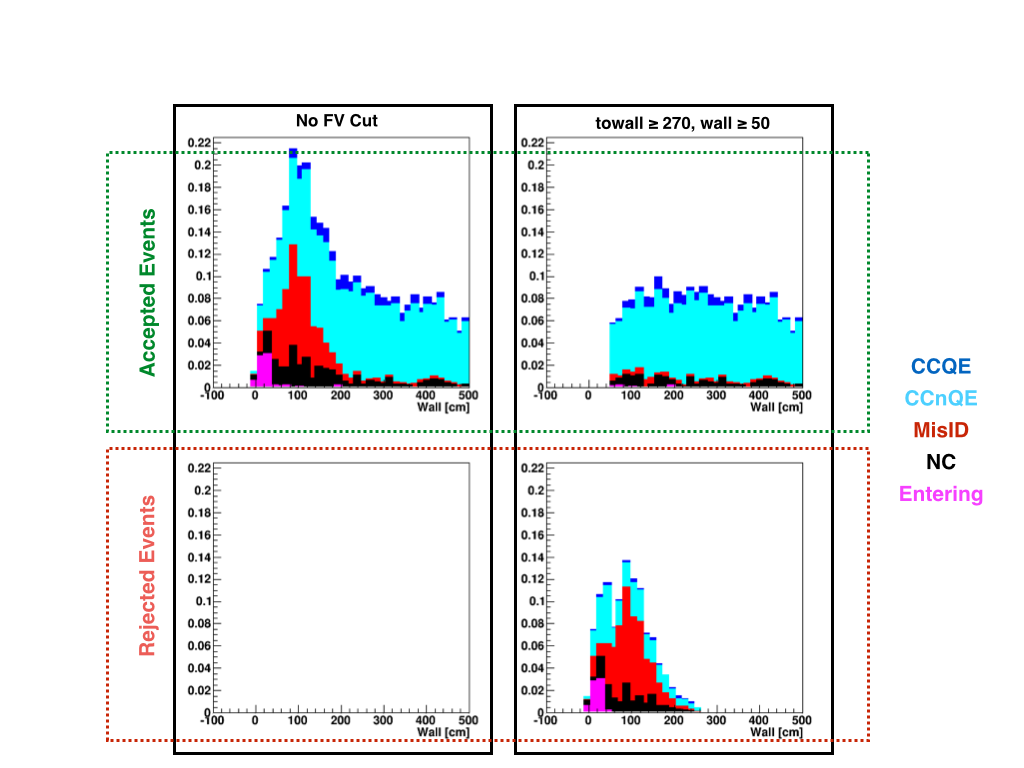
\includegraphics[width=0.65\textwidth]{plt_nuepi_wall}
%    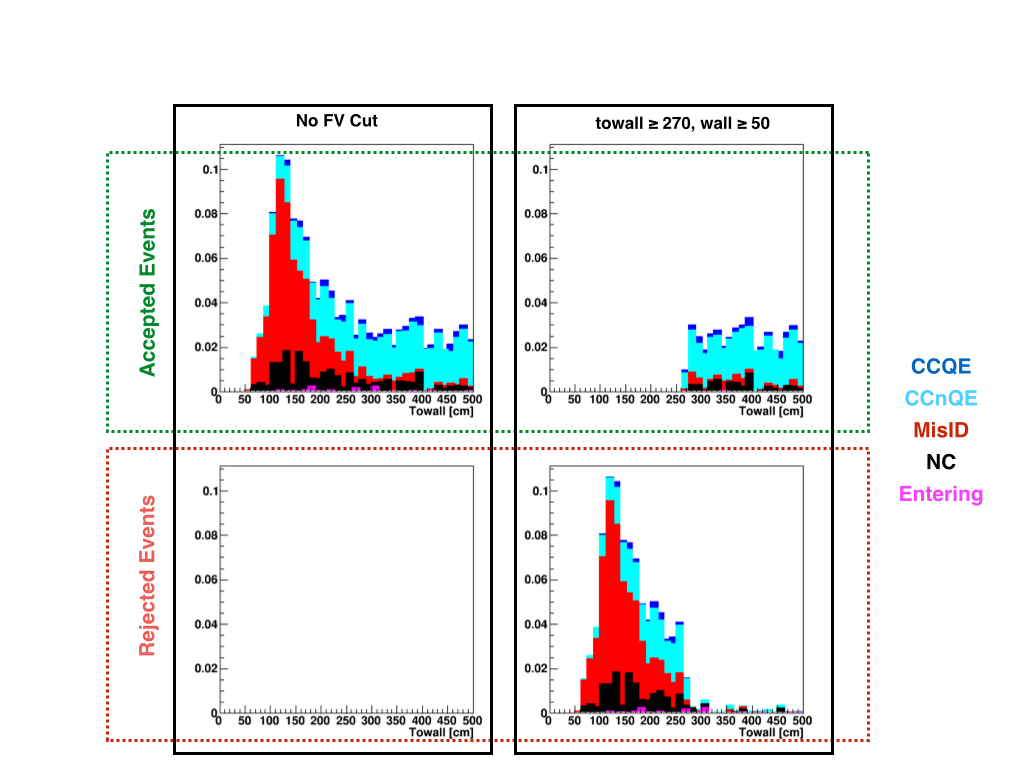
\includegraphics[width=0.65\textwidth]{plt_nuepi_towall}
%  \end{center}
%  \caption{Plots of the various MC categories that pass the T2K \nue CC1R$\pi$
%  topological cuts binned in \wall (top) and \towall (bottom).  Left
%  column shows the distribution with FV cut values at $0 cm$.  Right column
%  shows the distributions at the optimized cut values. Upper row shows the
%  events that pass the given FV cuts, bottom row shows the events that fail the
%  FV cuts. 
%  }
%  \label{fig:nue1rpitowall}
%\end{figure}
%
%
%\begin{figure}[h]
%  \begin{center}
%    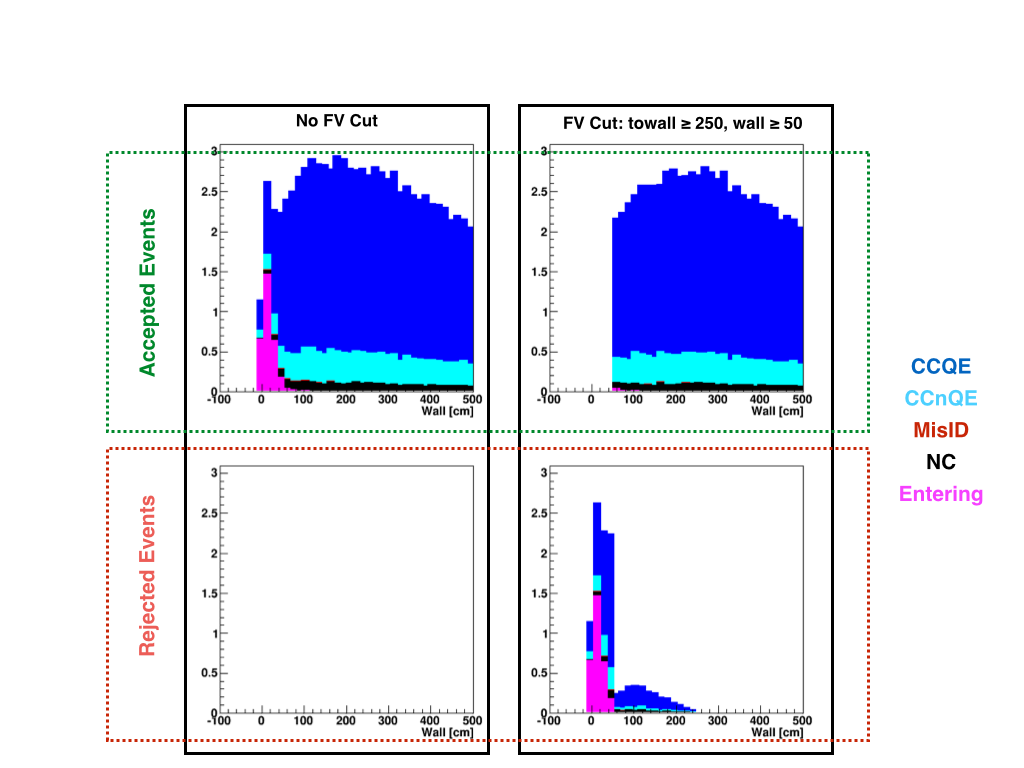
\includegraphics[width=0.65\textwidth]{plt_numu_wall}
%    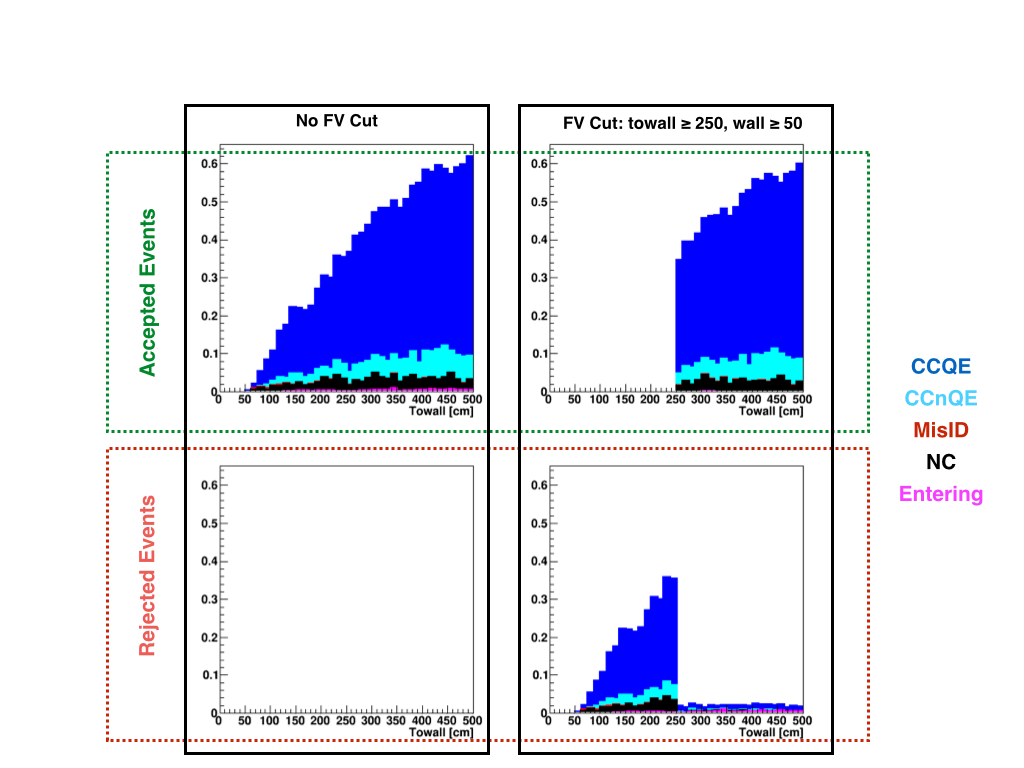
\includegraphics[width=0.65\textwidth]{plt_numu_towall}
%  \end{center}
%  \caption{Plots of the various MC categories that pass the T2K \numu
%  topological cuts binned in \wall (top) and \towall (bottom).  Left
%  column shows the distribution with FV cut values at $0 cm$.  Right column
%  shows the distributions at the optimized cut values. Upper row shows the
%  events that pass the given FV cuts, bottom row shows the events that fail the
%  FV cuts. 
%  }
%  \label{fig:numutowall}
%\end{figure}
%



